%%%%%%%%%%%%%%%%%%%%%%%%%%%%%%%%%%%%%%%%%%%%%%%%%%%%%%%%%%%%%%%%%%%%%%%%%%%%%%
% CS240: Programming in C
% Copyright 2016 Pejman Ghorbanzade <pejman@ghorbanzade.com>
% Creative Commons Attribution-ShareAlike 4.0 International License
% https://github.com/ghorbanzade/UMB-CS240-2016S/blob/master/LICENSE
%%%%%%%%%%%%%%%%%%%%%%%%%%%%%%%%%%%%%%%%%%%%%%%%%%%%%%%%%%%%%%%%%%%%%%%%%%%%%%

\def \topDirectory {.}
\def \resDirectory {\topDirectory/src/c/main/ls11}
\def \texDirectory {\topDirectory/src/tex}
\def \styDirectory {\texDirectory/sty}
\def \cfgDirectory {\texDirectory/cfg}
\def \imgDirectory {\texDirectory/img}

\documentclass[compress]{beamer}
%\mode<presentation>
%\usetheme{default}

\usepackage{\styDirectory/directives}
%%%%%%%%%%%%%%%%%%%%%%%%%%%%%%%%%%%%%%%%%%%%%%%%%%%%%%%%%%%%%%%%%%%%%%%%%%%%%%
% CS114: Introduction to Programming in Java
% Copyright 2015 Pejman Ghorbanzade <mail@ghorbanzade.com>
% Creative Commons Attribution-ShareAlike 4.0 International License
% https://github.com/ghorbanzade/UMB-CS114-2015F/blob/master/LICENSE
%%%%%%%%%%%%%%%%%%%%%%%%%%%%%%%%%%%%%%%%%%%%%%%%%%%%%%%%%%%%%%%%%%%%%%%%%%%%%%

\course{id}{CS240}
\course{name}{Programming in C}
\course{venue}{Mon/Wed, 5:30 PM - 6:45 PM}
\course{semester}{Spring 2016}
\course{department}{Department of Computer Science}
\course{university}{University of Massachusetts Boston}

\instructor{name}{Pejman Ghorbanzade}
\instructor{title}{}
\instructor{position}{Student Instructor}
\instructor{email}{pejman@cs.umb.edu}
\instructor{phone}{617-287-6419}
\instructor{office}{S-3-124B}
\instructor{office-hours}{Mon/Wed 16:00-17:30}
\instructor{address}{University of Massachusetts Boston, 100 Morrissey Blvd., Boston, MA}

\usepackage{\styDirectory/beamerthemePejman}
\doc{number}{11}
%\setbeamertemplate{footline}[text line]{}

\begin{document}

\prepareCover

\section{Pointers}

\subsection{Pointers and Arrays}

\begin{slide}
	\begin{block}{Introduction}

	Pointers and arrays are closely tied together and almost similar in practice.
	Any operation that can be achieved by array subscripting can also be achieved by pointers.

	\inputminted[
		fontsize=\footnotesize,
		firstline=14,
		lastline=17,
		linenos
	]{c}{\resDirectory/array1.c}

	\end{block}
\end{slide}

\begin{slide}
	\begin{block}{Accessing Array Elements}

	If pointer $p$ points to element $x_i$ of array $a$, pointer $p+1$ points to element $x_{i + 1}$ of array $a$.

	\inputminted[
		fontsize=\footnotesize,
		firstline=14,
		lastline=19,
		linenos
	]{c}{\resDirectory/array1.c}

	\end{block}
\end{slide}

\begin{slide}
	\begin{block}{Remember}

	Name of an array is a synonym for the location of the initial element.

	\inputminted[
		fontsize=\footnotesize,
		firstline=14,
		lastline=19,
		linenos
	]{c}{\resDirectory/array2.c}

	\end{block}
\end{slide}

\begin{slide}
	\begin{block}{Differences}

	\inputminted[
		fontsize=\footnotesize,
		firstline=15,
		lastline=23,
		linenos
	]{c}{\resDirectory/string1.c}

	\end{block}
	\begin{block}{Moral Point}

	A pointer to a character is not a character; it is a pointer.

	\end{block}
\end{slide}

\subsection{Pointers and Functions}

\begin{slide}
	\begin{block}{Exercise}

	Write a function \texttt{strcpy(char *s, char *t)} that copies the string \texttt{t} to the string \texttt{s}.
	You may assume that the destination string is larger than the source.

	\end{block}
\end{slide}

\begin{slide}
	\begin{block}{Solution 1}

	\inputminted[
		fontsize=\scriptsize,
		firstline=10,
		linenos
	]{c}{\resDirectory/strcpy1.c}

	\end{block}
\end{slide}

\begin{slide}
	\begin{block}{Solution 2}

	\inputminted[
		fontsize=\scriptsize,
		firstline=10,
		linenos
	]{c}{\resDirectory/strcpy2.c}

	\end{block}
\end{slide}

\begin{slide}
	\begin{block}{Solution 3}

	\inputminted[
		fontsize=\scriptsize,
		firstline=10,
		linenos
	]{c}{\resDirectory/strcpy3.c}

	\end{block}
\end{slide}

\begin{slide}
	\begin{figure}
	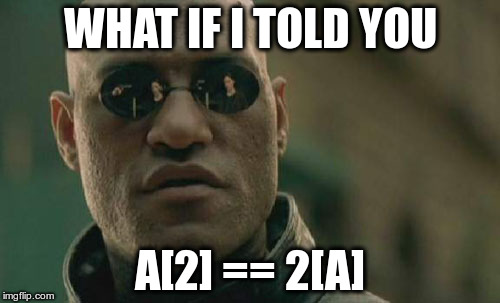
\includegraphics[width=0.8\textwidth]{\imgDirectory/array.jpg}
	\end{figure}
\end{slide}

\begin{slide}
	\begin{block}{Exercise}

	Write a function with the following signature that reverses a given array of integer.

	\begin{terminal}
	void reverse(int *array, int size);
	\end{terminal}

	\end{block}
\end{slide}

\begin{slide}
	\begin{block}{Solution}

	\inputminted[
		fontsize=\scriptsize,
		firstline=10,
		lastline=25,
		linenos
	]{c}{\resDirectory/reverse.c}

	\end{block}
\end{slide}

\begin{slide}
	\begin{block}{Solution}


	\inputminted[
		fontsize=\scriptsize,
		firstline=27,
		linenos
	]{c}{\resDirectory/reverse.c}

	\end{block}
\end{slide}

\begin{slide}
	\begin{block}{Exercise}

	Write a function with the following signature that multiples a square matrix $m$ by itself, given a pointer to element $m_{1,1}$.

	\begin{terminal}
	void matrix(int *m, int size);
	\end{terminal}

	\end{block}
\end{slide}

\begin{slide}
	\begin{block}{Solution}

	\inputminted[
		fontsize=\scriptsize,
		firstline=17,
		lastline=28,
		linenos
	]{c}{\resDirectory/matrix.c}

	\end{block}
\end{slide}

\begin{slide}
	\begin{block}{Solution}

	\inputminted[
		fontsize=\scriptsize,
		firstline=30,
		lastline=38,
		linenos
	]{c}{\resDirectory/matrix.c}

	\end{block}
\end{slide}

\begin{slide}
	\begin{block}{Solution}

	\inputminted[
		fontsize=\scriptsize,
		firstline=40,
		lastline=48,
		linenos
	]{c}{\resDirectory/matrix.c}

	\end{block}
\end{slide}

\begin{slide}
	\begin{block}{Solution}

	\inputminted[
		fontsize=\scriptsize,
		firstline=50,
		lastline=61,
		linenos
	]{c}{\resDirectory/matrix.c}

	\end{block}
\end{slide}

\begin{slide}
	\begin{block}{Solution}

	\inputminted[
		fontsize=\scriptsize,
		firstline=63,
		lastline=74,
		linenos
	]{c}{\resDirectory/matrix.c}

	\end{block}
\end{slide}

\begin{slide}
	\begin{figure}
	
\includegraphics[width=0.6\textwidth]{\imgDirectory/pulp.jpg}
	\end{figure}
\end{slide}

\end{document}
